\section{Recursive Functions}
\label{sec:recurs}
\begin{frame}<beamer>
    \frametitle{Outline}
    \tableofcontents[currentsection]
\end{frame}

\begin{frame}[fragile]{Recursive Function (1)}
\begin{itemize}
	\item {We already know that function is allowed to call any other function}
	\item {Function is allowed to call itself, this is called \textbf{recursive}}
	\item {It looks like following}
\end{itemize}
\begin{lstlisting}
int func2(int n);
int func1(int n)
{
   int a = 2*func1(n-2);
   ...
   int b = func2(n-3);
   return (a+b);
}
\end{lstlisting}

\begin{itemize}
	\item {Noticed that ``func1'' has been called inside ``func1''}
	\item {The scale of the problem decreases in each calling}
\end{itemize}

\end{frame}

\begin{frame}[fragile]{Recursive Function: how it works (1)}
\vspace{-0.28in}
\begin{columns}
\begin{column}{0.48\linewidth}
\begin{lstlisting}
long fact(int n)
{
   long a = 0;
   if (n < 0)
     a = 0;
   else if(n == 1 || n == 0)
    a  = 1;
   else
    a = n*fact(n-1);
    
   return a;
}
\end{lstlisting}
\end{column}
\begin{column}{0.45\linewidth}
\begin{lstlisting}
long fact(int n)
{
   long a = 1;
   int i = 0;
   if(n < 0)
     return 0;
   for(i = n; i > 0; i--)
   {
      a = a*i;
   }
   return a;
}
\end{lstlisting}
\end{column}
\end{columns}
\vspace{-0.16in}
\begin{lstlisting}
int main()
{
   int n = 4, b = 0;
   b = fact(n);
   printf("fact(%d) = %d\n", n, b);
   return 0;
}
\end{lstlisting}
\end{frame}

\begin{frame}[fragile]{Recursive Function: how it works (2)}
\vspace{0.1in}
\begin{itemize}
	\item {``fact'' calls itself until the \textbf{bottom} is reached}
	\item {Noticed that the scale of the problem decreases gradually}
	\item {Advantage: simple}
	\item {Darkside: requires a lot of memory}
\end{itemize}
\vspace{0.2in}
\begin{figure}
	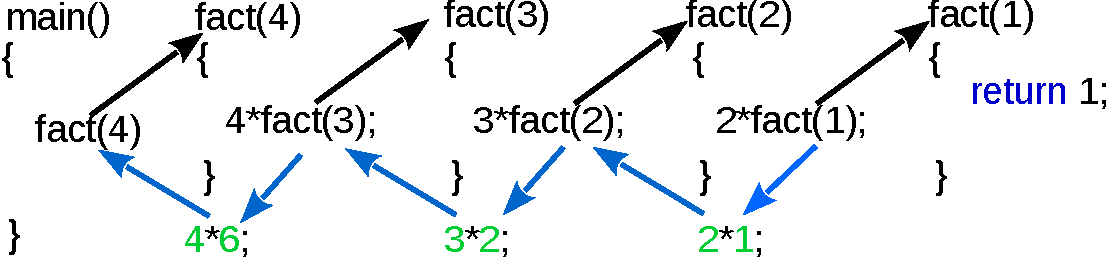
\includegraphics[width=0.95\linewidth]{figs/recurs.pdf}
\end{figure}
\begin{itemize}
	\item {Suggesion: try to avoid to use recursive function}
\end{itemize}
\end{frame}

\begin{frame}{Recursive Function: Hanoi Tower Problem}
\begin{itemize}
	\item {One is allowed to move one disc from one beam to another a day}
	\item {Move all 64 discs from beam A to C}
\end{itemize}
%\vspace{0.2in}
\begin{figure}
	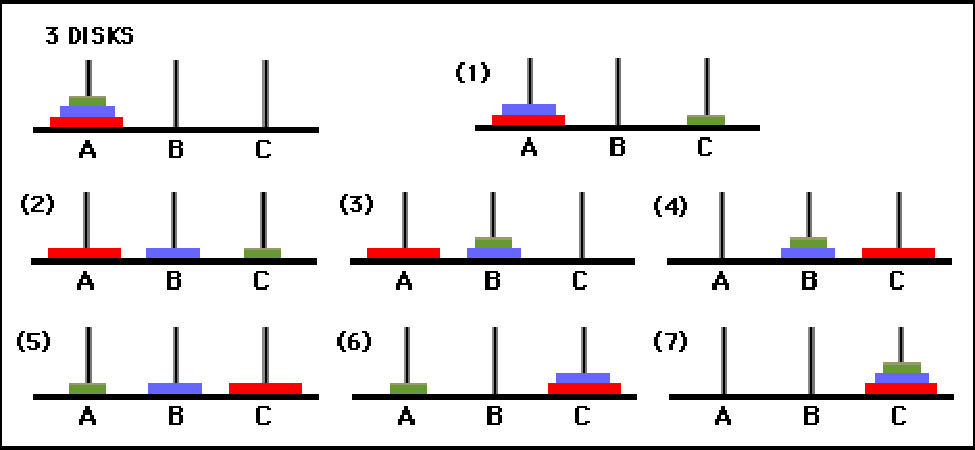
\includegraphics[width=0.85\linewidth]{figs/hanoi.pdf}
\end{figure}
\begin{itemize}
	\item {\textbf{It would not be fulfilled even till the end of this world!!}}
\end{itemize}
\end{frame}

\begin{frame}[fragile]{Source code for Hanoi Tower (1)}
\vspace{-0.15in}
\begin{lstlisting}[xleftmargin=0.02\linewidth, linewidth=0.85\linewidth]
#include <stdio.h>
void hanoi(int n, char b1, char b2, char b3)
{
    if(n == 1)
    {
        printf("%c ----> %c \n", b1, b3);
    }else if(n == 2)
    {
        printf("%c ----> %c\n", b1, b2);
        printf("%c ----> %c\n", b1, b3);
        printf("%c ----> %c\n", b2, b3);
    }else{
        hanoi(n-1, b1, b3, b2);
        printf("%c ----> %c\n", b1, b3);
        hanoi(n-1, b2, b1, b3);
    }
}
\end{lstlisting}
\vspace{-0.1in}

\end{frame}

\begin{frame}[fragile]{Source code for Hanoi Tower (2)}
\vspace{-0.15in}
\begin{lstlisting}[firstnumber=19, xleftmargin=0.02\linewidth, linewidth=0.85\linewidth]
int main()
{
   int n = 20;
   printf("Input n: ");
   scanf("%d", &n);
   hanoi(n, 'A', 'B', 'C');
}
\end{lstlisting}
\begin{enumerate}
	\item {Move top \textbf{n-1} plates from \textcolor{red}{\textbf{A}} to \textcolor{red}{\textbf{B}} via \textcolor{red}{\textbf{C}}}
	\item {Move the \textbf{bottom one} to \textcolor{red}{\textbf{C}}}
	\item {Move \textbf{n-1} plates from \textcolor{red}{\textbf{B}} to \textcolor{red}{\textbf{C}} via \textcolor{red}{\textbf{A}}}
\end{enumerate}
\end{frame}